
\documentclass[10pt,letterpaper]{article}

\usepackage[letterpaper,margin=0.70in,headheight=22pt,headsep=16pt,footskip=24pt]{geometry}
\usepackage[T1]{fontenc}
\usepackage[utf8]{inputenc}
\usepackage{lmodern}
\usepackage{microtype}
\usepackage{xcolor}
\usepackage{graphicx}
\usepackage{booktabs}
\usepackage{array}
\usepackage{tabularx}
\usepackage{longtable}
\usepackage{amsmath,amssymb}
\usepackage{tikz}
\usetikzlibrary{arrows.meta,positioning,calc,shapes.geometric,decorations.pathreplacing,fit}
\usepackage{enumitem}
\usepackage{fancyhdr}
\usepackage{titlesec}
\usepackage{caption}
\usepackage{listings}
\usepackage{xurl}
\usepackage[hidelinks]{hyperref}
\usepackage{lastpage}
\usepackage{float}
\usepackage{placeins}

\definecolor{FStatRed}{HTML}{A00000}
\definecolor{FStatGray}{HTML}{555555}
\definecolor{FStatBlue}{HTML}{144E8C}
\definecolor{LightGray}{HTML}{F3F3F3}
\definecolor{MidGray}{HTML}{D9D9D9}
\definecolor{DarkText}{HTML}{1A1A1A}
\definecolor{GoodGreen}{HTML}{2B7A2B}
\definecolor{WarnOrange}{HTML}{A65E00}

\renewcommand{\familydefault}{\sfdefault}
\setlength{\parindent}{0pt}
\setlength{\parskip}{5pt}
\renewcommand{\arraystretch}{1.15}
\sloppy
\setlist[itemize]{leftmargin=1.2em,itemsep=2pt,topsep=2pt}
\setlist[enumerate]{leftmargin=1.4em,itemsep=2pt,topsep=2pt}

\titleformat{\section}{\Large\bfseries\color{DarkText}}{}{0pt}{}[\vspace{-3pt}\color{FStatRed}\titlerule]
\titleformat{\subsection}{\large\bfseries\color{DarkText}}{}{0pt}{}
\titleformat{\subsubsection}{\normalsize\bfseries\color{DarkText}}{}{0pt}{}

\newcommand{\code}[1]{\texttt{\detokenize{#1}}}
\newcommand{\apicode}[1]{\texttt{\detokenize{#1}}}
\newcommand{\yes}{\textcolor{GoodGreen}{Yes}}
\newcommand{\no}{\textcolor{FStatGray}{No}}
\newcolumntype{Y}{>{\raggedright\arraybackslash}X}
\newcolumntype{L}[1]{>{\raggedright\arraybackslash}p{#1}}
\newcolumntype{C}[1]{>{\centering\arraybackslash}p{#1}}
\captionsetup{font=small,labelfont=bf}

\lstdefinestyle{shell}{
  basicstyle=\ttfamily\footnotesize,
  breaklines=true,
  columns=fullflexible,
  frame=single,
  rulecolor=\color{MidGray},
  backgroundcolor=\color{LightGray},
  keepspaces=true,
  showstringspaces=false
}
\lstdefinestyle{cstyle}{
  basicstyle=\ttfamily\footnotesize,
  breaklines=true,
  columns=fullflexible,
  frame=single,
  rulecolor=\color{MidGray},
  backgroundcolor=\color{LightGray},
  keepspaces=true,
  showstringspaces=false
}
\lstset{style=shell}

\newcommand{\notebox}[1]{%
  \vspace{4pt}\noindent\fcolorbox{FStatBlue}{LightGray}{%
  \begin{minipage}{0.965\linewidth}%
  \textbf{Note:} #1%
  \end{minipage}}\vspace{4pt}}

\newcommand{\importantbox}[1]{%
  \vspace{4pt}\noindent\fcolorbox{FStatRed}{LightGray}{%
  \begin{minipage}{0.965\linewidth}%
  \textbf{Important:} #1%
  \end{minipage}}\vspace{4pt}}

\newcommand{\field}[1]{\texttt{\detokenize{#1}}}
\newcommand{\dB}{\,\mathrm{dB}}


\pagestyle{fancy}
\fancyhf{}
\fancyhead[L]{\small PilotProxy-DS001}
\fancyhead[C]{\small CUDA F-Statistic DTV Pilot Detector v0.2.0.dev0}
\fancyhead[R]{\small Product Specification}
\fancyfoot[L]{\small PilotProxy-DS001 v1.6}
\fancyfoot[C]{\small West Virginia University}
\fancyfoot[R]{\small Page \thepage\ of \pageref{LastPage}}
\renewcommand{\headrulewidth}{0.8pt}
\renewcommand{\headrule}{\hbox to\headwidth{\color{FStatRed}\leaders\hrule height \headrulewidth\hfill}}
\renewcommand{\footrulewidth}{0.8pt}
\renewcommand{\footrule}{\hbox to\headwidth{\color{FStatRed}\leaders\hrule height \footrulewidth\hfill}}

\title{PilotProxy CUDA F-Statistic DTV Pilot Detector v0.2.0.dev0\\Product Specification}
\author{West Virginia University}
\date{PilotProxy-DS001 v1.6 \\ July 19, 2026}

\begin{document}
\thispagestyle{fancy}
{\sffamily
\begin{minipage}[t]{0.39\textwidth}
  {\fontsize{24}{26}\selectfont\bfseries\color{FStatRed}PilotProxy}\par
  {\small PilotProxy-DS001 v1.6, July 19, 2026}
\end{minipage}
\hfill
\begin{minipage}[t]{0.58\textwidth}
  \raggedleft
  {\fontsize{18}{20}\selectfont\bfseries CUDA F-Statistic DTV Pilot Detector v0.2.0.dev0}\par
  {\small Product Specification}
\end{minipage}
}

\vspace{0.14in}

\begin{minipage}[t]{0.48\textwidth}
\section*{Introduction}
PilotProxy measures ATSC 1.0 DTV pilot tones with a fixed-point CUDA F-statistic detector. We use the narrow pilot as a proxy for a DTV data shelf that may lie below the broadband noise floor. The package includes the CUDA kernel, a public C API, Python wrappers, a precomputed ATSC weight bank, and a GNU Radio validation testbench.

The detector core is receiver-independent. The standalone testbench supplies its own reference front end, while the CHIME workflow supplies instrument metadata and packed telescope data through a separate adapter. This boundary keeps receiver assumptions out of the CUDA kernel without claiming that real-data operation is instrument-independent.

ATSC A/53 Part 2 specifies that the 8-VSB pilot is approximately 11.3 dB below the average data-signal power \cite{atsc_a53_part2_2011}. We record the positive magnitude of this relationship as \(\mathrm{pilot\_below\_data\_db}=11.3\dB\). Host software uses it to convert one-bin pilot excess to an equivalent DTV data-shelf SNR.

\subsection*{Features}
\begin{itemize}
  \item Fixed-point CUDA detector for ATSC 1.0 pilot excess.
  \item Fixed 128-sample detector rows using packed complex 4+4 bit input.
  \item Three matched-filter terms: target pilot bin, lower reference bin, upper reference bin.
  \item Exact \code{uint64} target/reference power readback.
  \item Synthetic-evaluator detection by rational fixed-point threshold comparison; no division in that mask path.
  \item Synthetic-evaluator threshold coordinate is DTV shelf SNR in dB.
  \item The corresponding kernel threshold coordinate is a fixed-point F-statistic half-threshold.
  \item GNU Radio ATSC 1.0 waveform generation, audit, AWGN injection, quantization, and SNR evaluation.
  \item Physical-channel helpers and shipped weights for U.S. UHF channels 14-36.
\end{itemize}
\end{minipage}
\hfill
\begin{minipage}[t]{0.48\textwidth}
\section*{PilotProxy Facts Table}
\small
\begin{tabularx}{\linewidth}{|>{\bfseries}L{0.43\linewidth}|Y|}
\hline
\multicolumn{2}{|c|}{\bfseries Core Specifics}\\ \hline
Package version & 0.2.0.dev0 (unreleased) \\ \hline
Kernel version & 1.0.0 \\ \hline
Primary function & Measure ATSC 1.0 pilot excess and estimate the corresponding data-shelf SNR \\ \hline
Input data & Packed complex int4, one complex sample per \code{int8_t} \\ \hline
Detector window & 128 packed complex samples \\ \hline
Weight terms & 3: target, lower reference, upper reference \\ \hline
Reference bins & Two total reference bins \\ \hline
Raw statistic & \(F=2P_t/(P_{r1}+P_{r2})\) \\ \hline
Raw/basic pilot excess & \(\rho=F-1\); positive raw excess begins at \(F>1\) \\ \hline
Kernel outputs & \code{num=P_t}, \code{den=P_r1+P_r2}, and \code{mask} \\ \hline
Power accumulation & \code{uint64} \\ \hline
\multicolumn{2}{|c|}{\bfseries User-Facing Controls}\\ \hline
Target selection & \code{physical_channel} or \code{dtv_pilot_mhz} selects precomputed weights \\ \hline
Frame size & \code{frame_size_samples}; positive multiple of 128 \\ \hline
Synthetic threshold & \code{threshold_snr_shelf_db}; converted by evaluator host software \\ \hline
\multicolumn{2}{|c|}{\bfseries Reference Testbench}\\ \hline
Reference ADC rate & 800 MS/s real input \\ \hline
Reference band & 400-800 MHz \\ \hline
PFB & 4-tap, 2048-point real-input PFB \\ \hline
Usable coarse channels & 1024 positive-frequency channels \\ \hline
Coarse-channel spacing & 390.625 kHz \\ \hline
Fine detector-bin width & 3051.7578125 Hz \\ \hline
Default physical channel & 14; 470--476 MHz band, pilot at 470.309441 MHz \\ \hline
Shipped weight range & Physical channels 14-36 \\ \hline
\multicolumn{2}{|c|}{\bfseries Implementation}\\ \hline
CUDA dot-product path & DP4A production path; scalar integer validation path \\ \hline
Default block threads & 64 \\ \hline
Default grid cap & 4096 blocks \\ \hline
Default weight placement & Shared-memory preload enabled \\ \hline
Execution policy & Device-affine, default stream \\ \hline
\end{tabularx}
\end{minipage}

\vfill
{\small\color{FStatGray}Unreleased v0.2.0.dev0. Synthetic thresholds are distinct from the current CHIME $F>\mu_0$ mask; $F>1$ is the basic raw convention. Measure performance on the target system.}

\newpage
\tableofcontents
\newpage

\section{General Description}

The DTV data shelf occupies most of a nominal 6 MHz channel, but the ATSC pilot is narrow. Therefore, we measure the pilot against two nearby reference bins and use that excess to estimate the equivalent data-shelf SNR. This estimate is conditional on the stated bandwidth, pilot-to-data relationship, and pilot-capture efficiency.

The CUDA kernel implements only the fixed-point measurement. It receives a row-major detector matrix, three packed weight vectors, and a rational half-threshold. It returns accumulated powers and a mask. Host software supplies the ATSC frequencies, dB conversions, receiver geometry, and physical-channel interpretation.


\begin{figure}[H]
\centering
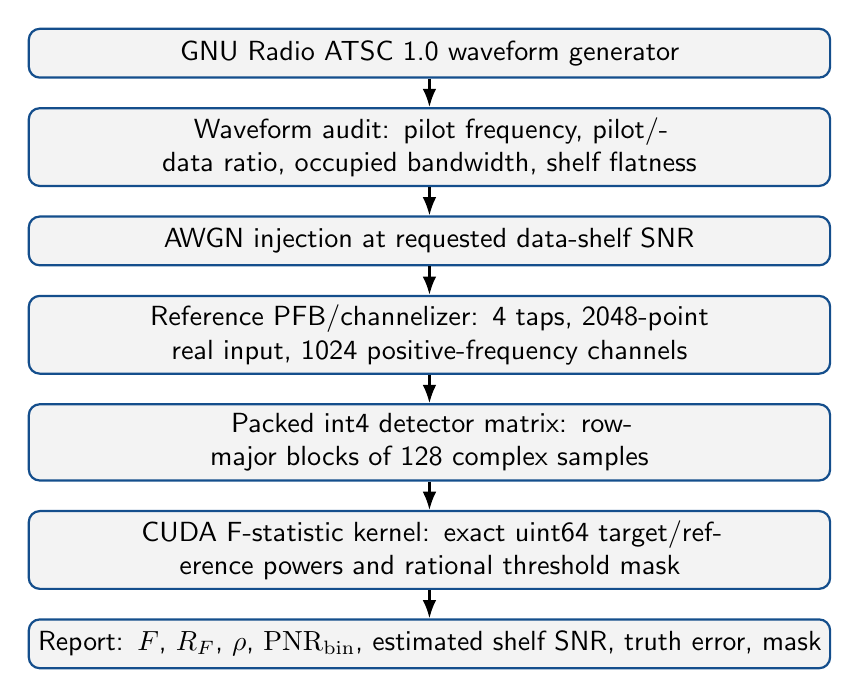
\begin{tikzpicture}[node distance=0.36cm,>=Latex]
\tikzstyle{block}=[rectangle,rounded corners,draw=FStatBlue,thick,fill=LightGray,minimum height=0.62cm,text width=0.82\linewidth,align=center]
\node[block] (a) {GNU Radio ATSC 1.0 waveform generator};
\node[block,below=of a] (b) {Waveform audit: pilot frequency, pilot/data ratio, occupied bandwidth, shelf flatness};
\node[block,below=of b] (c) {AWGN injection at requested data-shelf SNR};
\node[block,below=of c] (d) {Reference PFB/channelizer: 4 taps, 2048-point real input, 1024 positive-frequency channels};
\node[block,below=of d] (e) {Packed int4 detector matrix: row-major blocks of 128 complex samples};
\node[block,below=of e] (f) {CUDA F-statistic kernel: exact uint64 target/reference powers and rational threshold mask};
\node[block,below=of f] (g) {Report: $F$, $R_F$, $\rho$, $\mathrm{PNR}_{\mathrm{bin}}$, estimated shelf SNR, truth error, mask};
\draw[->,thick] (a) -- (b);
\draw[->,thick] (b) -- (c);
\draw[->,thick] (c) -- (d);\draw[->,thick] (d) -- (e);
\draw[->,thick] (e) -- (f);
\draw[->,thick] (f) -- (g);
\end{tikzpicture}
\caption{Standalone validation flow. The included reference front end connects a generated ATSC waveform to the same packed-input detector contract used by the CUDA kernel.}
\label{fig:validation_flow}
\end{figure}


\section{Signal Definitions}

\subsection{Raw F-Statistic}

For one evaluated frame, the kernel accumulates three powers:
\begin{equation}
  P_t,\qquad P_{r1},\qquad P_{r2}.
\end{equation}
The target term \(P_t\) is centered on the ATSC pilot. The lower and upper reference terms, \(P_{r1}\) and \(P_{r2}\), sample the nearby non-pilot floor. We form the raw F-statistic as
\begin{equation}
  \boxed{F=\frac{2P_t}{P_{r1}+P_{r2}}.}
\end{equation}
The production \code{NumDen} API writes:
\begin{equation}
  \code{num}=P_t,\qquad \code{den}=P_{r1}+P_{r2}.
\end{equation}
Therefore, host code must use \(F=2\,\code{num}/\code{den}\). Using \(\code{num}/\code{den}\) would omit the factor of two in the detector definition.

\subsection{Pilot Excess and PNR}

The raw F-statistic level is:
\begin{equation}
  R_F=10\log_{10}F.
\end{equation}
This level is not the physical pilot-to-noise ratio because \(F=1\) is the uncorrected no-excess point. We define the corresponding raw pilot excess as
\begin{equation}
  \boxed{\rho=F-1.}
\end{equation}
The one-bin pilot-excess PNR is:
\begin{equation}
  \boxed{\mathrm{PNR}_{\mathrm{bin},dB}=10\log_{10}(F-1).}
\end{equation}
If \(F\leq 1\), this logarithm is undefined. JSON reports encode the value as \code{null}.

\subsection{DTV Shelf SNR}

We define the DTV data-shelf SNR as the ATSC data-and-sync shelf power spectral density relative to the non-DTV noise floor. The pilot is not part of the shelf numerator. For the standard conversion, we compute
\begin{equation}
  \boxed{\mathrm{SNR}_{\mathrm{shelf},dB}=
  \mathrm{PNR}_{\mathrm{bin},dB}
  -10\log_{10}\left(\frac{B_{\mathrm{DTV}}}{B_{\mathrm{bin}}}\right)
  +\mathrm{pilot\_below\_data\_db}
  -10\log_{10}(\eta_p).}
\end{equation}
The default constants are:
\begin{equation}
 B_{\mathrm{DTV}}=6\,\mathrm{MHz},\quad
 B_{\mathrm{bin}}=3051.7578125\,\mathrm{Hz},\quad
 \mathrm{pilot\_below\_data\_db}=11.3\dB,
 \quad \eta_p=1.0.
\end{equation}
For these constants, the bandwidth spreading term is
\begin{equation}
  10\log_{10}\left(\frac{6\times 10^6}{3051.7578125}\right)=32.936\dB.
\end{equation}


\begin{figure}[H]
\centering
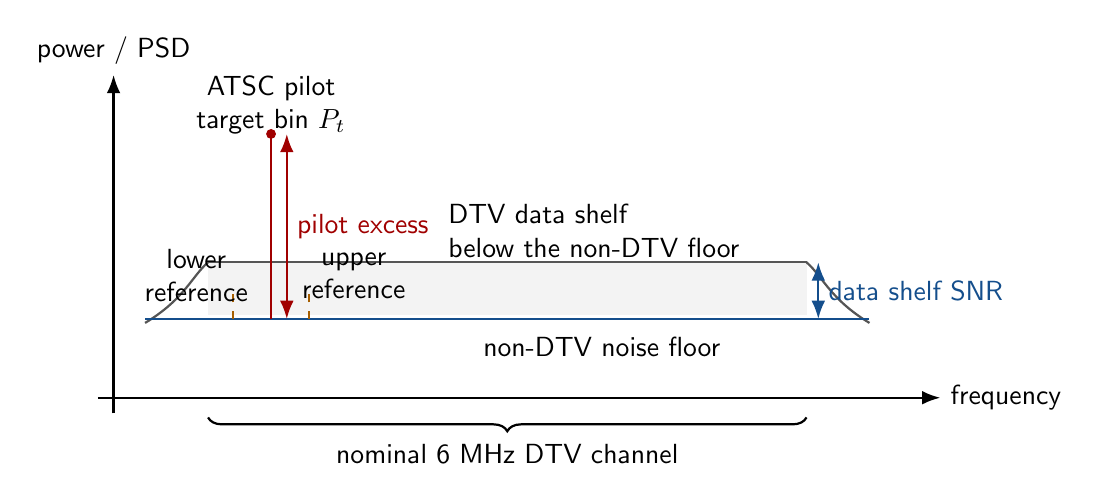
\begin{tikzpicture}[x=1.0cm,y=1.0cm,>=Latex]
  \draw[->,thick] (-0.2,0) -- (10.5,0) node[right]{frequency};
  \draw[->,thick] (0,-0.2) -- (0,4.1) node[above]{power / PSD};
  \draw[fill=LightGray,draw=none] (1.2,1.05) rectangle (8.8,1.72);
  \draw[thick,FStatGray] (1.2,1.72) -- (8.8,1.72);
  \draw[thick,FStatGray] (0.4,0.95) .. controls (0.9,1.25) and (1.0,1.55) .. (1.2,1.72);
  \draw[thick,FStatGray] (8.8,1.72) .. controls (9.0,1.55) and (9.1,1.25) .. (9.6,0.95);
  \draw[thick,FStatBlue] (0.4,1.0) -- (9.6,1.0);
  \draw[thick,FStatRed] (2.0,1.0) -- (2.0,3.35);
  \draw[fill=FStatRed,draw=FStatRed] (2.0,3.35) circle (0.055);
  \draw[dashed,thick,WarnOrange] (1.52,1.0) -- (1.52,1.35);
  \draw[dashed,thick,WarnOrange] (2.48,1.0) -- (2.48,1.35);
  \draw[<->,thick,FStatRed] (2.20,1.0) -- (2.20,3.35) node[midway,right]{pilot excess};
  \draw[<->,thick,FStatBlue] (8.95,1.0) -- (8.95,1.72) node[midway,right]{data shelf SNR};
  \draw[decorate,decoration={brace,mirror,amplitude=5pt},thick] (1.2,-0.25) -- (8.8,-0.25)
    node[midway,below=6pt]{nominal 6 MHz DTV channel};
  \node[align=center] at (2.0,3.72) {ATSC pilot\\target bin $P_t$};
  \node[align=center] at (1.05,1.55) {lower\\reference};
  \node[align=center] at (3.05,1.55) {upper\\reference};
  \node[align=left] at (6.1,2.12) {DTV data shelf\\below the non-DTV floor};
  \node[align=left] at (6.2,0.65) {non-DTV noise floor};
\end{tikzpicture}
\caption{Signal definitions used by the detector. The kernel compares the target pilot bin with two local reference bins. Host software then converts the measured one-bin excess to an equivalent 6 MHz data-shelf SNR under the stated calibration constants.}
\label{fig:spectrum_definitions}
\end{figure}


\section{Threshold Interpretation}

For synthetic threshold tests, the user supplies \code{threshold_snr_shelf_db}. Host software converts this shelf-SNR threshold to the raw F-statistic coordinate and then to the rational half-threshold used by the kernel:

\begin{align}
\mathrm{PNR}_{\mathrm{bin,thr},dB} &= S_{\mathrm{shelf,thr},dB} - \mathrm{pilot\_below\_data\_db} + 10\log_{10}(B_{\mathrm{DTV}}/B_{\mathrm{bin}})+10\log_{10}(\eta_p),\\
\rho_{\mathrm{thr}} &= 10^{\mathrm{PNR}_{\mathrm{bin,thr},dB}/10},\\
F_{\mathrm{thr}} &= 1+\rho_{\mathrm{thr}},\\
T_{\mathrm{half}} &= \frac{F_{\mathrm{thr}}}{2}=\frac{N_{\mathrm{half}}}{D_{\mathrm{half}}}.
\end{align}
The CUDA kernel evaluates:
\begin{equation}
  P_t D_{\mathrm{half}} > N_{\mathrm{half}}(P_{r1}+P_{r2}).
\end{equation}
Exact equality is not a positive detection. The rational-half API and the CHIME positive-excess path both use a strict greater-than comparison.


\notebox{We independently recomputed the following example from the checked-in conversion code. For a \(-26\dB\) shelf-SNR threshold and the included reference geometry, \(\mathrm{PNR}_{\mathrm{bin}}=-4.363988\dB\), \(F_{\mathrm{thr}}=1.36610123\), and \(T_{\mathrm{half}}\approx0.68305\).}

\section{Channel and Frequency Support}

The shipped weight bank covers U.S. physical channels 14 through 36. The eCFR assigns channel 14 to 470--476 MHz and channel 36 to 602--608 MHz \cite{ecfr_73603}. Following the ATSC pilot offset, the default channel-14 target is 470.309441 MHz.

\begin{longtable}{|C{0.13\linewidth}|C{0.18\linewidth}|C{0.20\linewidth}|C{0.33\linewidth}|}
\hline
\textbf{Physical channel} & \textbf{Lower edge} & \textbf{Pilot} & \textbf{Coarse index: ascending reference / shipped CHIME}\\ \hline
14 & 470.000 MHz & 470.309441 MHz & 179 / 843\\ \hline
21 & 512.000 MHz & 512.309441 MHz & 287 / 735, references edge wrapped\\ \hline
36 & 602.000 MHz & 602.309441 MHz & 517 / 505\\ \hline
\end{longtable}

The first index is the standalone ascending-frequency reference coordinate. The second is the post-spectral-sense-normalization coordinate stored in the shipped CHIME manifest and printed by \code{pilot-proxy list-channels}. The nominal references are two fine bins below and above the target. For physical channel 21, the target lies near a coarse-channel boundary. The generated layout therefore wraps the lower reference across the circular coarse-channel spectrum while preserving the two-bin offset. Detection and validation reports copy the selected manifest row into \field{selected_weight_layout}, so this placement remains visible in each result.

\section{Receiver Integration Contract}

The CUDA detector core does not interpret receiver metadata. A receiver adapter must supply the following metadata and arrays above the kernel boundary:
\begin{itemize}
  \item \code{DetectorCoreProfile}: locked kernel contract, including \(K=128\), \(N=3\), int4 packed input, uint64 powers, and rational half-threshold input.
  \item \code{ReceiverProfile}: RF band, channelizer geometry, spectral sense, frame size, input-stream count, quantization defaults, fine-bin ENBW, and pilot-capture efficiency.
  \item \code{stream_map}: stream-index metadata for feed, polarization, beam, or other receiver paths.
  \item \code{check-profile}, \code{check-layout}, \code{make-weights}, and \code{chime-run} consume the applicable profile or stream-map records. The standalone \code{detect} command selects shipped weights from its sidecar or channel flag, while \code{evaluate-snr} uses the fixed testbench geometry.
\end{itemize}

After this adaptation, the kernel receives only packed rows and packed weights, and it writes uint64 powers and a mask. For one selected DTV channel, the adapter constructs
\begin{equation}
N_{\mathrm{rows}} = N_{\mathrm{input\ streams}}\,
\frac{\mathrm{frame\_size\_samples}}{128}.
\end{equation}
The default combine mode is an incoherent power sum over streams. We sum the powers before forming the statistic:
\begin{equation}
F = \frac{2\sum_r P_{t,r}}{\sum_r P_{r1,r}+\sum_r P_{r2,r}},
\end{equation}
where \(r\) indexes detector rows. The result schema names this rule \code{all_rows_summed_before_ratio}. Per-stream packing remains available for integration diagnostics, but the combined detection path forms one \(F\) only after summing all selected rows.

The checked-in \code{chime_dtv_fengine_v1} receiver profile uses 16,384 channelized samples per input stream. This is the planned CHIME Engine upgrade profile used by the repository's analysis and tests; it is not a claim about the currently deployed correlator frame. The software does not infer one universal value from HDF5 metadata: \code{chime-run} accepts an explicit per-run frame-size override, while \code{chime-scan} takes \code{nfft} from the DataTrawl instrument configuration. Operators must verify and record the resolved value for each real-data product.

\section{Result Schema and Mask Convention}

Detector and synthetic SNR-evaluator JSON outputs include a versioned \field{result_schema} object with \code{schema_version=pilot_proxy_result_v2}. This object records the statistic definitions, layout metadata, calibration constants, threshold fields, fixed-point contract, and mask convention needed to interpret those results. Audit, quantization, summary, injection, and CHIME products use their own documented top-level schemas rather than this object.

The fixed-point contract records:
\begin{itemize}
  \item \field{detector_window_samples=128};
  \item \field{reference_offset_bins=2} nominally, with \field{skipped_guard_bins=1} and adaptive placement metadata copied from the weight manifest;
  \item \field{packed_complex_bits=8};
  \item \field{sample_bits_per_component=4};
  \item \field{power_accumulator=uint64}.
\end{itemize}

For products that average masked data, we use exclusion masking:
\begin{equation}
\bar{P}_{\mathrm{after}} =
\frac{\sum_b P_b(1-M_b)}{\sum_b (1-M_b)}.
\end{equation}
Here \(M_b=1\) excludes block \(b\). We divide by the number of retained blocks rather than replacing excluded blocks with zeros.

The CHIME mask does not use a mean estimated from CANFAR data. For each fixed-point weight row, the weight norms define the flat-floor null point
\begin{equation}
\mu_0=\frac{2\,\lVert w_t\rVert^2}{\lVert w_{r1}\rVert^2+\lVert w_{r2}\rVert^2}.
\end{equation}
The basic uncorrected convention would call \(F>1\) positive excess. The current implementation instead masks a valid CHIME frame only when \(F>\mu_0\), evaluated by integer cross multiplication. This correction accounts for unequal norms introduced by int4 weight quantization; it is not an empirical RFI threshold and does not establish an operational false-positive rate.

\section{Reference PFB and Detector Resolution}

The standalone testbench uses the following reference channelizer:
\begin{itemize}
  \item real ADC sample rate: 800 MS/s;
  \item modeled band: 400 MHz bandwidth;
  \item PFB: 4 taps, 2048-point real input;
  \item usable positive-frequency channels: 1024;
  \item coarse-channel spacing: \(800\,\mathrm{MHz}/2048=390.625\,\mathrm{kHz}\);
  \item fine detector-bin spacing: \(390.625\,\mathrm{kHz}/128=3051.7578125\,\mathrm{Hz}\).
\end{itemize}
These values define the tested reference geometry. In particular, the default SNR conversion uses the resulting 3051.7578125 Hz fine-bin width. A receiver with a different effective noise bandwidth must provide its own value.

\section{Data Format}

Each input sample is one \code{int8_t} containing a packed complex int4 value:
\begin{equation}
  \text{bits }[7:4]=\mathrm{real},\qquad \text{bits }[3:0]=\mathrm{imag}.
\end{equation}
We decode each nibble as two's-complement signed int4 with range \([-8,7]\). The generated weights use the symmetric range \([-7,7]\), which avoids the unmatched negative endpoint when generating detector ROMs.

Input matrices are row-major:
\begin{equation}
  \mathrm{d\_in}[m,k]=\mathrm{d\_in}[mK+k],\qquad K=128.
\end{equation}
For batched input:
\begin{equation}
  \mathrm{d\_in}[b,m,k]=\mathrm{d\_in}[(bM+m)K+k].
\end{equation}

\section{Fixed-Point Sizing}

The int4 growth bound sets the detector window to 128 samples. We conservatively bound one real or imaginary complex-product component by 128 per tap. Therefore, 128 taps give an absolute component bound of 16,384, which fits in signed 16-bit storage. A 256-sample power-of-two window could reach 32,768 and exceed the positive signed-int16 limit. Under the same bound, one magnitude-squared term fits in \code{uint32}, and the configured block power sum fits in \code{uint64}.

\section{C API Summary}

\small
\begin{longtable}{|L{0.54\linewidth}|L{0.38\linewidth}|}
\hline
\textbf{Function} & \textbf{Purpose}\\ \hline
\apicode{FStat_GetSpecs} & Query detector-window samples, number of weight terms, component bits, and reference-bin offset.\\ \hline
\apicode{FStat_GetFeatures} & Query DP4A use, uint64 accumulation use, and CUDA block size.\\ \hline
\apicode{FStat_GetOptimizationFeatures} & Query weight-lane placement and grid cap.\\ \hline
\apicode{FStat_GetVersion} & Query the locked kernel version.\\ \hline
\apicode{FStat_LastError} & Read the last CUDA/API error recorded by the calling thread.\\ \hline
\apicode{FStat_Create} / \apicode{FStat_Create_Batch} & Create default-stream device-affine handle.\\ \hline
\apicode{FStat_Compute_NumDen_Mask_RationalHalf} & Production detection path without overflow counter.\\ \hline
\apicode{FStat_Compute_NumDen_Mask_RationalHalf_WithOverflowCount} & Production detection path with rational multiplication overflow counter.\\ \hline
\apicode{FStat_Compute_Powers_U64} & Integer diagnostic/reference readback of all three power terms.\\ \hline
\apicode{FStat_Compute_DiagnosticFloat} & Diagnostic float32 ratio output; not the primary validation path.\\ \hline
\apicode{FStat_Destroy} & Destroy handle.\\ \hline
\end{longtable}
\normalsize

A zero reference denominator cannot define \(F\). The kernel therefore sets the mask to zero. Unchecked C and Python conversion helpers return zero pilot excess for this case. The checked C helper exposes the invalid denominator; Python callers must inspect \code{den} or \field{p_ref_sum_u64} before interpreting the conversion.

\section{Build and Validation}

We recommend a source-tree installation for kernel development:
\begin{lstlisting}[style=shell]
PYTHONPATH=src python -m pilot_proxy.cli --help
python -m pip install -e ".[test]"              # Python tests
python -m pip install -e ".[cuda,test,plot]"    # GPU and plot workflow
\end{lstlisting}
Build the CUDA kernel:
\begin{lstlisting}[style=shell]
make build-kernel   # SM auto-detected; pass SM=<arch> to override
\end{lstlisting}
Run Python tests and kernel tests on a CUDA-capable machine:
\begin{lstlisting}[style=shell]
PYTHONPATH=src python -m pytest tests -q
make -C cuda test DP4A=1   # SM auto-detected
\end{lstlisting}

\begin{figure}[H]
\centering
\IfFileExists{../generated/dtv_snr_eval/dtv_snr_sweep.png}{%
\includegraphics[width=0.88\linewidth]{../generated/dtv_snr_eval/dtv_snr_sweep.png}
\caption{Example standalone shelf-SNR sweep for the stated test configuration: \(-60\dB\) to \(0\dB\) in 3 dB steps, 10 independent Python-noise trials per point, one input stream, and no plot smoothing. The diagonal is an input-equals-output reference. The curves compare the unquantized floating-point model with the selected packed-int4 fixed-point backend. Ten trials per point are a functional example, not a publication-level uncertainty estimate.}
}{%
\fbox{\parbox{0.86\linewidth}{\centering The optional generated SNR sweep figure was not found. Run the validation sweep and plot workflow to create \code{generated/dtv_snr_eval/dtv_snr_sweep.png}.}}
\caption{Example standalone shelf-SNR sweep for the stated test configuration: \(-60\dB\) to \(0\dB\) in 3 dB steps, 10 independent Python-noise trials per point, one input stream, and no plot smoothing. The diagonal is an input-equals-output reference. The curves compare the unquantized floating-point model with the selected packed-int4 fixed-point backend. Ten trials per point are a functional example, not a publication-level uncertainty estimate.}
}
\label{fig:snr_sweep_10trial}
\end{figure}

\notebox{The current \code{plot-results} helper labels its fixed-point series ``GPU fixed-point'' even when the result was produced with \code{--detector-backend cpu-reference}. For a CPU-reference result, plot the CSV directly or relabel the curve ``CPU fixed-point'' and retain the recorded backend with the figure.}

The repository provides separate Python, CPU, CUDA, and GNU Radio checks. A release record should state which checks ran, on which commit, and on which host. CUDA and GNU Radio results cannot be inferred from a Python-only run and must be measured on a suitable target machine before release.

\section{Limitations}

\begin{itemize}
  \item Installed wheels and sdists carry the weight bank and \code{configs/} resources; default-resource commands such as \code{list-channels} work outside the repository. Workflows that use repository-relative generated paths, helper scripts, a second Python interpreter, or the CUDA build require a checkout or explicit paths. The CUDA kernel is not packaged and builds from the cloned source tree.
  \item The CUDA API is default-stream only.
  \item The shipped weight bank covers physical channels 14-36 only.
  \item Standalone validation models ATSC 1.0 signals generated with GNU Radio. It does not by itself validate telescope performance.
  \item The CHIME baseband workflow is implemented in \code{pilot_proxy.chime} and documented by its runbooks. The checked-in 16,384-sample profile represents the planned Engine upgrade interface and remains subject to run-metadata verification.
  \item Receiver profiles define an adapter contract; they do not establish that a telescope pipeline has been deployed or validated.
  \item The CHIME mask uses $F>\mu_0$, where $\mu_0$ comes from fixed weight norms. It is not a threshold fitted to telescope null statistics, and no operational false-positive rate is claimed.
  \item The kernel measures pilot excess. It does not decode an ATSC transport stream or prove that every excess is DTV.
  \item Standard conversion uses the ATSC 11.3 dB relationship. Any calibrated override must be recorded with the result that used it.
\end{itemize}

\begin{thebibliography}{9}
\bibitem{atsc_a53_part2_2011} Advanced Television Systems Committee, \emph{ATSC Digital Television Standard, Part 2: RF/Transmission System Characteristics}, A/53 Part 2:2011, 15 December 2011. \url{https://www.atsc.org/wp-content/uploads/2021/04/A53-Part-2-2011.pdf}
\bibitem{ecfr_73603} Electronic Code of Federal Regulations, 47 CFR \S 73.603, \emph{Numerical designation of television channels}. \url{https://www.ecfr.gov/current/title-47/chapter-I/subchapter-C/part-73/subpart-E/section-73.603}
\bibitem{gnuradio_noise} GNU Radio Manual, \emph{gr::analog::noise\_source}, complex noise-source amplitude convention. \url{https://www.gnuradio.org/doc/doxygen/classgr_1_1analog_1_1noise__source.html}
\end{thebibliography}

\clearpage
\section{Revision History}
\begin{tabularx}{\linewidth}{|L{0.18\linewidth}|L{0.14\linewidth}|Y|}
\hline
\textbf{Date} & \textbf{Version} & \textbf{Revision}\\ \hline
July 19, 2026 & 1.6 & Corrected package state, threshold and mask scope, receiver-metadata consumers, coordinate-system labels, frame-size handling, installation prerequisites, and result-schema coverage. Distinguished the raw $F>1$ convention from the current norm-corrected $F>\mu_0$ CHIME rule.\\ \hline
July 3, 2026 & 1.5 & Updated for the \code{pilot-proxy} 0.2.0 development series. Packaged weight/config resources with console-script CLI; CUDA kernel remains a source-tree build; limitations refreshed (CHIME real-data subsystem ships separately; fixed weight-norm mask in place of telescope-null thresholds).\\ \hline
July 2, 2026 & 1.4 & Norm-corrected positive-excess mask: the mask compares against the exact H0 zero-point $\mu_0 = 2\,n_t/(n_l+n_u)$ set by the int4 weight norms (rule and product fields updated accordingly); runtime bundles carry the per-channel rational half-threshold $n_t:(n_l+n_u)$.\\ \hline
May 29, 2026 & 1.3 & Added receiver-profile integration contract, full stream-map example, and profile-driven weight generation.\\ \hline
May 29, 2026 & 1.2 & Regenerated for standalone \code{pilot-proxy} v0.1.0.  Added strict PNR/SNR terminology, physical channel support, calibration fields, strict JSON behavior, channel-21 edge-wrap handling, and source-tree release notes.\\ \hline
May 29, 2026 & 1.1 & Standalone DTV scope; instrument-specific material removed.\\ \hline
May 29, 2026 & 1.0 & Initial kernel product specification.\\ \hline
\end{tabularx}

\end{document}
